\documentclass[12pt]{article}
\setlength{\oddsidemargin}{0in}
\setlength{\evensidemargin}{0in}
\setlength{\textwidth}{6.5in}
\setlength{\parindent}{0in}
\setlength{\parskip}{\baselineskip}
\usepackage{amsmath,amsfonts,amssymb}
\usepackage{graphicx}
\usepackage[]{algorithmicx}
\usepackage{enumitem}
\usepackage{fancyvrb}
\usepackage{ wasysym }

\usepackage{fancyhdr}
\pagestyle{fancy}
\setlength{\headsep}{36pt}

\usepackage{hyperref}


\hypersetup{
    colorlinks=true,
    linkcolor=blue,
    filecolor=magenta,      
    urlcolor=blue,
}
\graphicspath{{F:/Users/sasha/Documents/Summer 2020/Algo/hw 3b}}
\newcommand{\makenonemptybox}[2]{%
%\par\nobreak\vspace{\ht\strutbox}\noindent
\item[]
\fbox{% added -2\fboxrule to specified width to avoid overfull hboxes
% and removed the -2\fboxsep from height specification (image not updated)
% because in MWE 2cm is should be height of contents excluding sep and frame
\parbox[c][#1][t]{\dimexpr\linewidth-2\fboxsep-2\fboxrule}{
  \hrule width \hsize height 0pt
  #2
 }%
}%
\par\vspace{\ht\strutbox}
}
\makeatother

\begin{document}
\lhead{{\bf CSCI 3104, Algorithms \\ Homework 3B (45 points)} }
\rhead{Name: \fbox{Sasha Farhat% Place your name here and delete the next time
\phantom{ This is a really long name}} 
\\ ID: \fbox{105887541 % Place your ID here and delete the next time
\phantom{This is a student ID}} 
\\ {\bf Escobedo \& Jahagirdar\\ Summer 2020, CU-Boulder}}
\renewcommand{\headrulewidth}{0.5pt}

\phantom{Test}

\begin{small}
\textit{Advice 1}:\ For every problem in this class, you must justify your answer:\ show how you arrived at it and why it is correct. If there are assumptions you need to make along the way, state those clearly.
%\vspace{-3mm} 

\textit{Advice 2}:\ Verbal reasoning is typically insufficient for full credit. Instead, write a logical argument, in the style of a mathematical proof.\\
%\vspace{-3mm} 

\textbf{Instructions for submitting your solution}:
\vspace{-5mm} 

\begin{itemize}
	\item The solutions \textbf{should be typed}, we cannot accept hand-written solutions. Here's a short intro to \href{http://ece.uprm.edu/~caceros/latex/introduction.pdf}{\textbf{Latex}.}
	 \item In this homework we denote the asymptomatic \textit{Big-O} notation by $\mathcal{O}$ and \textit{Small-O} notation is represented as $o$. 
	\item We recommend using online Latex editor \href{https://www.overleaf.com/}{\textbf{Overleaf}}. Download the \textbf{.tex} file from Canvas and upload it on overleaf to edit.
	%todo add link of gradescope
	\item You should submit your work through \href{https://www.gradescope.com}{\textbf{Gradescope}}  only.
	\item If you don't have an account on it, sign up for one using your CU email. You should have gotten an email to sign up. If your name based CU email doesn't work, try the identikey@colorado.edu version. 
	\item Gradescope will only accept \textbf{.pdf} files (except for code files that should be submitted separately on Canvas if a problem set has them) and \textbf{try to fit your work in the box provided}. 
	\item You cannot submit a pdf which has less pages than what we provided you as Gradescope won't allow it.
   
\end{itemize}
\vspace{-4mm} 
\end{small}

\hrulefill
\pagebreak

\subsection*{Piazza threads for hints and further discussion}
\begin{center}
    \begin{tabular}{|c|}
    \hline
    Piazza Threads \\ [0.5ex] 
    \hline \hline 
    \href{https://piazza.com/class/ka2roz7rb9m3j4?cid=47}{Question 1}\\
    \href{https://piazza.com/class/ka2roz7rb9m3j4?cid=48}{Question 2}\\
    \hline
    \end{tabular}
\end{center}

\textbf{Recommended reading} \\ 
\textbf{Greedy Algorithms}: Ch. 16 →  16.1, 16.2, 16.3; Ch. 2 →  2.1, 2.2

\pagebreak

\begin{enumerate}

	 \item{\itshape $(7.5 \times 2 = 15$ pts$)$ In this question we will look at the \textbf{Interval scheduling} problem. The problem consists of a set of tasks. Each of these tasks need to be executed in a specific time interval. Two tasks are set to be compatible if their time intervals do not overlap. The goal is to find the maximum set of compatible tasks so that as many tasks possible can be executed. For example consider the case of just three tasks\\
	 }
	 \begin{center}
    \begin{tabular}{|c|c|c|}
    \hline
    Task &  start time & end time\\ [0.5ex] 
    \hline \hline 
    Task 1 & 1 & 10 \\
    \hline
    Task 2 & 2 & 5 \\
    \hline
    Task 3 & 7 & 9 \\
    \hline
    \end{tabular} \\
   
\end{center}
{\itshape Here the set consisting of Task 2 and Task 3 is the set consisting of maximum number of compatible tasks. It is maximum because if we select Task 1, then we cannot select either Task 2 or Task 3 as both of them have overlapping intervals with Task 1.} 
 
	\begin{enumerate}[label=(\alph*)]
	 \item{\itshape 
	    Consider a greedy algorithm which always selects the shortest appointment first. Provide an example in tabular form with at least 5 tasks where this algorithm fails. List the
order in which the algorithm selects the intervals, and also write down a larger
subset of non-overlapping intervals than the subset output by the greedy algorithm. \\ \\
        \textbf{Note} \\
        A comment on level of justification  to help us understand your thinking, it is worth writing a little about the order in which the algorithm selects the tasks. For example, The algorithm consider tasks in the order [Task 3, Task 2, Task 1]: first the algorithm selects Task 3 because that is the shortest. Task 1 conflicts Task3, so it is removed. In the next step the shortest and only remaining Task 2 is selected.
	 }
	 \makenonemptybox{6in}{
	 Say we have the following Task Schedules:\\
	 \textbf{Task01}   01-10\\
	 \textbf{Task02}   02-05\\
	 \textbf{Task03}   07-09\\
	 \textbf{Task04}   05-08\\
	 \textbf{Task05}   08-11\\
	 \\
	 Considering a greedy algorithm which always selects the shortest appointment first, the algorith fails to maximize this interval scheduling. The algorithm considers all 5 tasks in this order [Task05, Task04, Task 03, Task02, Task 01]. \\
	 The algorithm will select Task03 first. \\
	 Task04 will be removed because it intervenes with Task03. \\
	 Task05 will also be removed because it intervenes with Task03. \\
	 Task01 is also removed because it intervenes with Task03. \\
	 The algorithm will select Task02 as the shortest and remaining schedule time. We end up with subset: \textbf{ [Task02, Task03].}
	 \\
	 \\
	 The algorithm fails here because the maximum task schedule subset is [Task02, Task04, Task05].
	 }
	 \clearpage
	 \item{\itshape
	 Consider a greedy algorithm which always selects the longest task first.
Provide an example in tabular form with at least 5 tasks where this algorithm fails. Show
the order in which the algorithm selects the intervals, and also show a larger subset
of non-overlapping intervals than the subset output by the greedy algorithm. \\
The \textbf{Note} provided in 2a applies here in terms of the level of explanation.
	 }
	  \makenonemptybox{6in}{
	   Say we have the following Task Schedules:\\
	 \textbf{Task01}   01-10\\
	 \textbf{Task02}   02-05\\
	 \textbf{Task03}   07-09\\
	 \textbf{Task04}   05-08\\
	 \textbf{Task05}   08-11\\
	 \\
	 Considering a greedy algorithm which always the longest task first, the algorithm fails to maximize this interval scheduling. The algorithm considers all 5 tasks in this order [Task05, Task04, Task 03, Task02, Task 01]. \\
	 The algorithm will select Task01 first. \\
	The algorithm will evaluate and remove Task05, Task04, Task 03, Task02. All of these tasks intervene with Task01.\\
	We are left with a task subset of \textbf{[Task01]}	  
	  }
	 
	\end{enumerate}
	\clearpage
	\item{\itshape $(10 \times 3 = 30)$
	In this question we'll consider weighted problems.
	}
	\begin{enumerate}[label=(\alph*)]
	\item{\itshape
	Consider the weighted interval scheduling problem. In this problem, the input is
a list of n tasks and weights, each of which is specified by $(start_i; end_i;w_i)$.
The goal is now to find a subset of the given intervals in which no two overlap and
to maximize the sum of the weights, rather than the total number of intervals in
your subset. That is, if your list has length $n$, the goal is to find $S \subseteq \{1, 2, ... n\}$
such that for any $i, j \in  S$, interval i and interval j do not overlap, and maximizing
$\sum_{i \in S} w_it_i$. Consider the greedy algorithm for interval scheduling from recitation, which selects the job with the earliest end time first. Give an example of weighted interval
scheduling with at least 5 intervals where this greedy algorithm fails. Show the
order in which the algorithm selects the intervals, and also show a higher-weight
subset of non-overlapping intervals than the subset output by the greedy algorithm.
The \textbf{Note} provided in 2a applies here in terms of the level of explanation.
	}
	\makenonemptybox{4.5in}{
	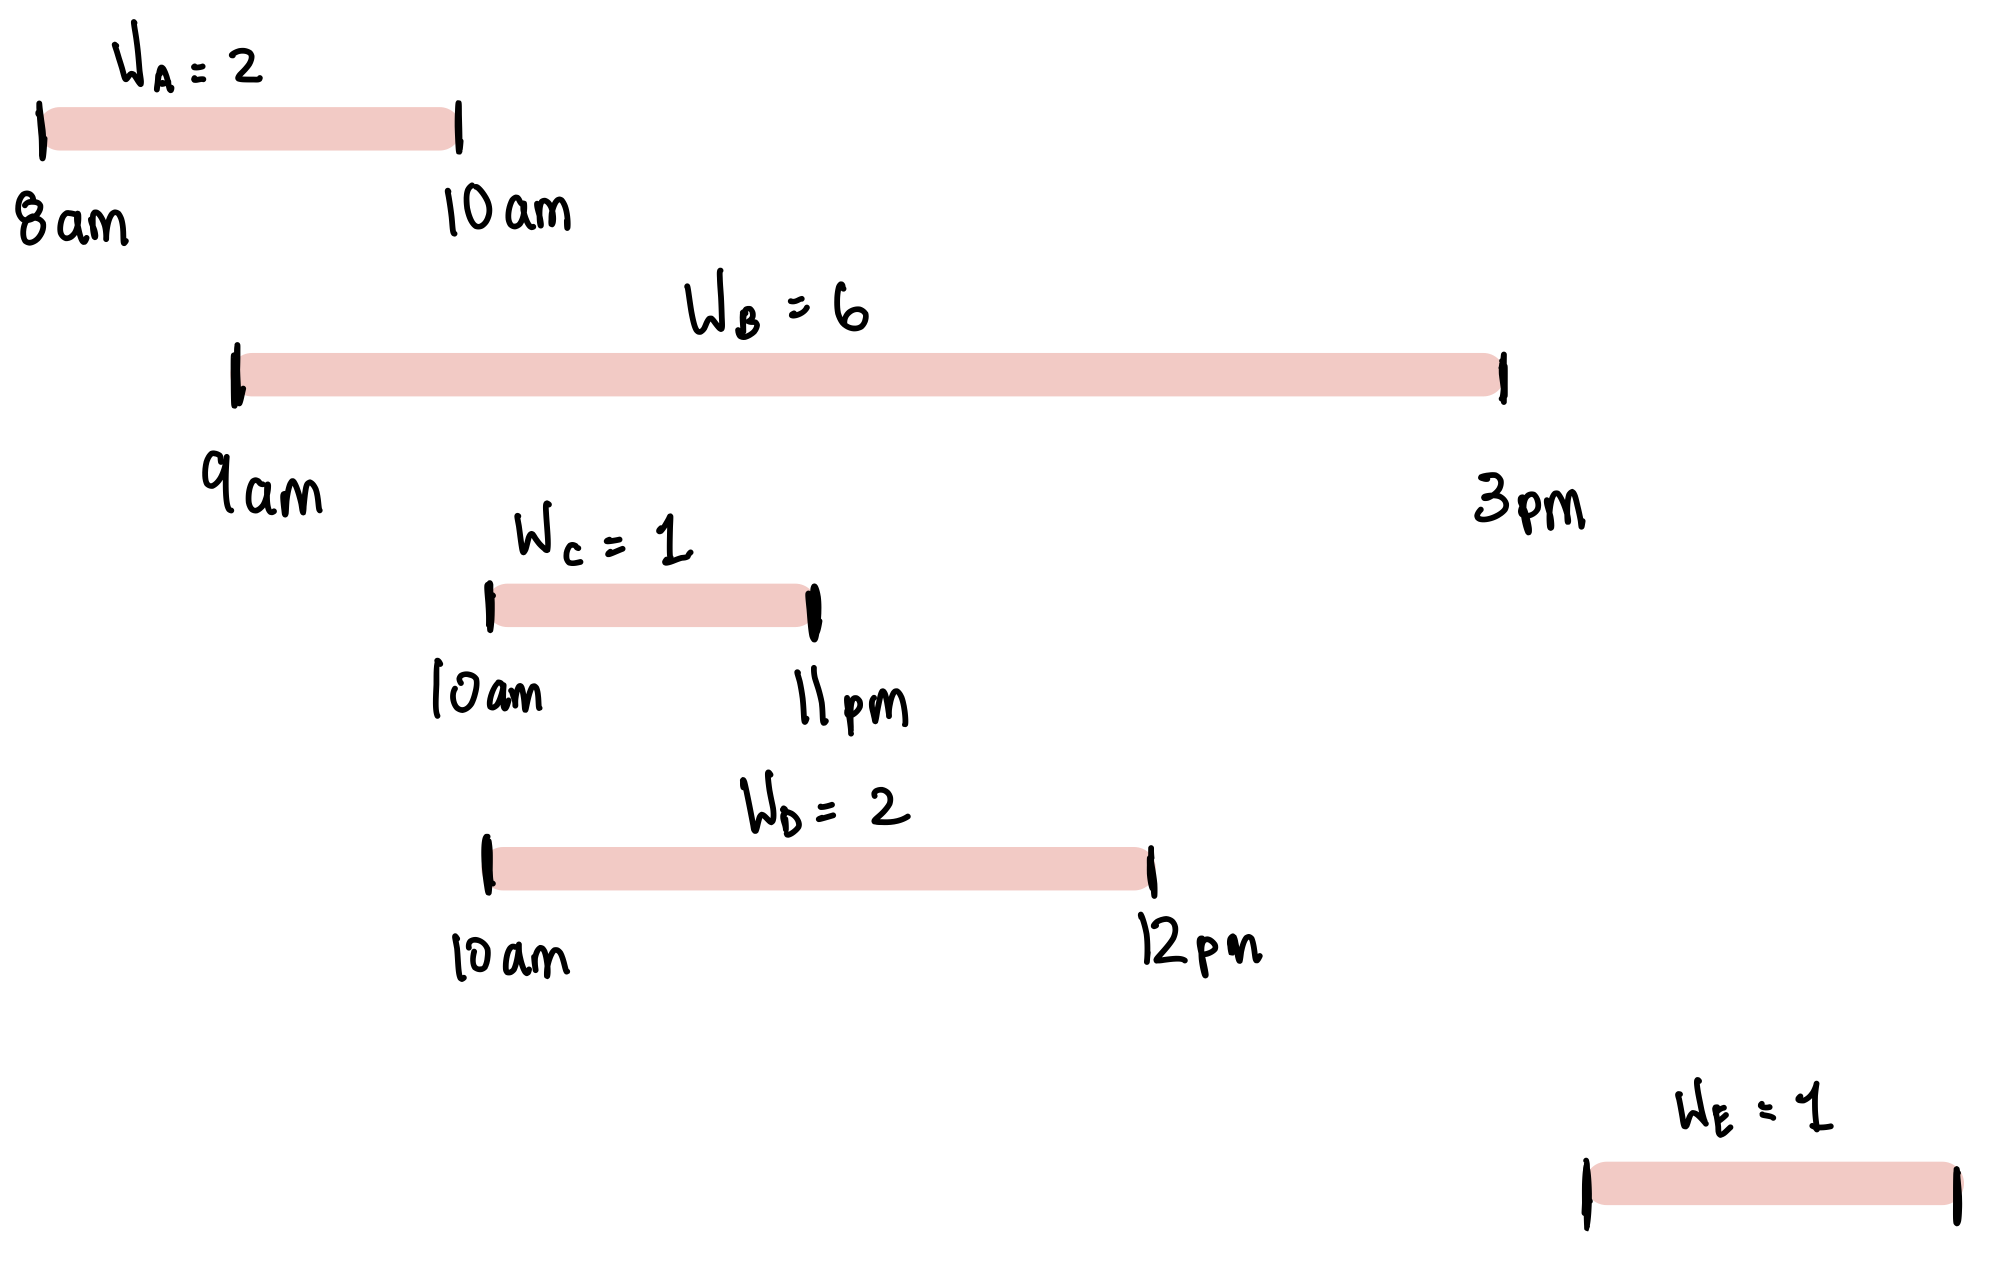
\includegraphics[scale=0.14]{answer2a.png}\\
	\\
	Considering a greedy algorithm which always the longest task first, the algorithm fails to maximize the weight in scheduling. The algorithm considers all 5 times in this order [$w_a,w_b,w_c,w_d,w_e$]. 
	 The algorithm will select $w_a$ first.
	 The algorithm will the remove $w_b$.
	THe algorithm will then select $w_c$ as the next schedule with the earliest end time.
	The algorithm will then evaluate $w_d$ and remove it.
	$w_e$ is the last of the intervals to be evaluated and selected. The greedy algorithm gives us the interval schedule : [$w_a,w_c, w_e)$]= 3. This algorithm fails to give the optimal weight. The optimal weight would be 7 with a schedule interval of [$w_c,w_e$].
	}
	\item{\itshape
	Consider the Knapsack problem: the input is a list of $n$ items, each with a
value and weight ($val_i;wt_i$), and a threshold weight $W$. All values and weights
are strictly positive. The goal is to select a subset $S$ of the items such that
$\sum_{i \in S} w_i t_i < W$ and maximizing $\sum_{i \in S} val_i$. (Note that, unlike change-making, here there is only one of each item, whereas in change-making you in principle
have an unlimited number of each type of coin.) Consider a greedy algorithm for
this problem which makes greedy choices as follows: among the remaining items,
choose the item of maximum value such that it will not make the total weight exceed the threshold $W$. Give an example of knapsack with at least 5 items where this
greedy algorithm fails. Show the order in which the algorithm selects the items,
and also show a higher-value subset whose weight does not exceed the threshold.
The \textbf{Note} provided in 2a applies here in terms of the level of explanation.
	}
	\makenonemptybox{5in}{}
	\item{\itshape
	Now consider the following algorithm for the knapsack problem. Call the relative
value of item $i$ the ratio $\frac{val_i}{wt_i}$. Consider the greedy algorithm which, among
the remaining items, chooses the item of maximum relative value such that it will
not make the total weight exceed the threshold $W$. Give an example of knapsack
where this greedy algorithm fails. Show the order in which the algorithm selects
the items, and also show a higher-value subset whose weight does not exceed the
threshold. The \textbf{Note} provided in 2a applies here in terms of the level of explanation.
	}
	\makenonemptybox{5.5in}{
	}
	\end{enumerate}

\clearpage
\item{\itshape \textbf{Extra Credit (5\% of total homework grade)}
    For this extra credit question, please refer the leetcode link provided below or click \href{https://leetcode.com/problems/minimum-cost-for-tickets/}{here}. Multiple solutions exist to this question ranging from brute force to the most optimal one. Points will be provided based on Time and Space Complexities relative to that of the most optimal solution.

    Please provide your solution with proper comments which carries points as well.}
    
   \url{https://leetcode.com/problems/minimum-cost-for-tickets/}

    % Paste your code in the verbatim tag below
\begin{verbatim}
Replace this text with your source code inside of the .tex document
\end{verbatim}	
	
	
\end{enumerate}



\end{document}


